\problemname{Backspace}

\illustration{0.45}{editor}{Bjarki í vandræðum}
% \begin{wrapfigure}{r}{0.35\textwidth}
%   \centering
%   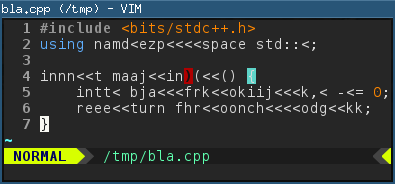
\includegraphics[width=0.93\textwidth]{editor.png}
% \end{wrapfigure}

Rétt áður en Forritunarkeppni Framhaldskólanna byrjaði ákvað Bjarki að
uppfæra tölvuna sína. Hann tók ekki eftir neinu þangað til að hann byrjaði að
skrifa fyrsta kóðann í uppáhalds ritlinum sínum Bim (Bjarki IMproved). Venjulega
þegar hann skrifar í ritlinum og ýtir á \emph{backspace} takkann þá strokast út einn
stafur til vinstri. En eftir uppfærsluna þá skrifast þess í stað út \textbf{\texttt{<}}. Hann er
búinn að prófa alla ritlana sem hann er með í tölvunni, Bmacs, Neobim, bjedit,
NoteBjad++, Subjark Text en þeir virðast allir hafa þetta vandamál. Hann hefur
ekki tíma til að vafra á netinu og finna lausn við þessu vandamáli svo hann
ákveður að taka málin í sínar hendur og einfaldlega redda þessu.

Hjálpaðu Bjarka að skrifa forrit sem tekur inn streng sem hann skrifaði og
prentar út strenginn eins og hann ætlaði að skrifa hann.

\section*{Inntak}
Fyrsta og eina línan inniheldur streng $S$ af lengd $N$ sem samanstendur
eingöngu af enskum lágstöfum og tákninu \texttt{<}.

\section*{Úttak}
Prentið út strenginn eins og Bjarki ætlaði að skrifa hann. Það er, sé
strengurinn prentaður út staf fyrir staf, þá táknar \texttt{<} útstrokun á
síðasta staf sem prentaður var út, eins og \emph{backspace} væri um að ræða.

\section*{Útskýring á sýnidæmum}
Í fyrsta sýnidæminu byrjar Bjarki að skrifa \texttt{a} sem hann strokar út,
skrifar \texttt{b} og \texttt{c} en strokar \texttt{c} síðan út. Úttakið verður því
\texttt{b}.
Í næsta sýnidæmi skrifar Bjarki \texttt{foss} en skrifar út síðustu tvo stafi
með \texttt{<}\texttt{<}, úttaksstrengurinn á þeim tímapunkti er því \texttt{fo}. Við
þetta er bætt \texttt{rritun} og er því úttakið \texttt{forritun}.
Í síðasta sýnidæminu er tvisvar skrifað \texttt{a} og strokað út. Í lokin er
skrifað \texttt{aa} og strokað tvisvar út með \texttt{<}\texttt{<}.

\section*{Stigagjöf}
Lausnin mun verða prófuð á miserfiðum inntaksgögnum, og er gögnunum skipt í
hópa eins og sýnt er í töflunni að neðan. Lausnin mun svo fá stig eftir því
hvaða hópar eru leystir.

\begin{tabular}{|l|l|l|l|}
\hline
Hópur & Stig & Inntaksstærð & Önnur skilyrði  \\ \hline
1     & 10         & $ 1 \le N \le 100$ & Strengurinn $S$ inniheldur eingöngu stafinn \texttt{a} og táknið \texttt{<}\\ \hline
2     & 10         & $ 1 \le N \le 100$ & Strengurinn $S$ inniheldur ekki tvö \texttt{<} í röð\\ \hline
3     & 40         & $ 1 \le N \le 100$ & \\ \hline
4     & 40         & $ 1 \le N \le 10^6$ & \\ \hline
\end{tabular}
